\documentclass[8pt]{beamer}

\usepackage[utf8]{inputenc}
\usepackage[T1]{fontenc}

\usepackage{longtable}
\usepackage{booktabs}

\usepackage{graphicx}
\usepackage{subfig}
\usepackage{floatrow}
\captionsetup{labelsep=period}

\usepackage[]{algorithm2e}
\SetKwRepeat{Do}{do}{while}

\usepackage{standalone}

\usepackage{amssymb, amsmath, mathrsfs, mathtools, dsfont, bbold, cancel}

\usetheme{ign}

\title{Classification et apprentissage statistique}
\subtitle{Supervisé et non-supervisé}
\author{Oussama ENNAFII}
\institute{ENSG}
\date{\today}

\begin{document}

	\begin{frame}[plain]
		\titlepage{}
	\end{frame}

	\section{Introduction}
		\begin{frame}{Classification: première définition}
			Champs lexical de classer:
			\begin{itemize}
				\item<2-> ranger,
				\item<3-> labeliser,
				\item<4-> catégoriser,
				\item<5-> hiérarchiser.
			\end{itemize}
			\uncover<6->{
				\begin{block}{Esquisse de définition}
					Classer: ranger \(n\) \textbf{objets} dans \(k\) \textbf{catégories} (avec \(k \ll n\)).
				\end{block}
			}
		\end{frame}
		
		\begin{frame}{Comment classer?}
			\begin{itemize}
					\item<1-> Comment caractériser un objet à classer?
					\item<2-> Comment sont-elle définit les catégories (ou classes) d'objets?
			\end{itemize}
		\end{frame}
	
	\section{Classification}
		\subsection{Exemples}
			\begin{frame}{Reconaissance d'objet}
				\begin{figure}[H]
					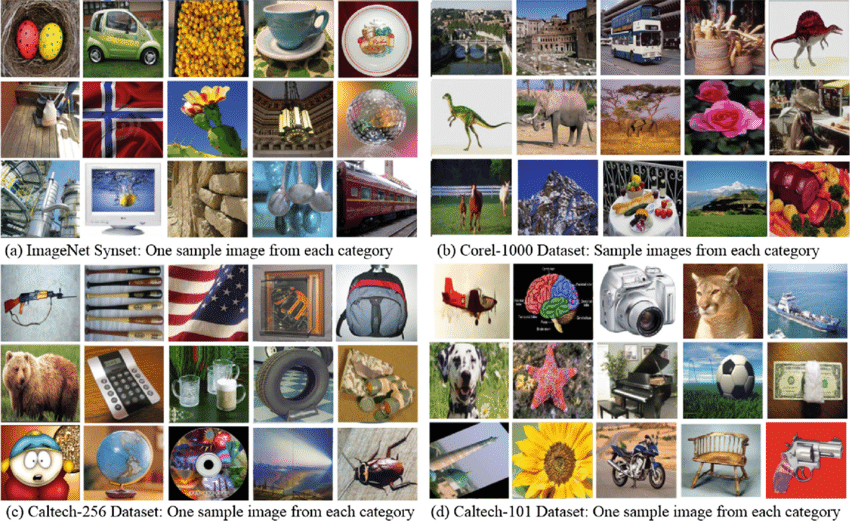
\includegraphics[width=.7\textwidth]{images/samples/image_datasets}
					\caption*{\tiny Exemples de base de données d'images~\cite{ahmed2017fusion}.}
				\end{figure}
			\end{frame}
			
			\begin{frame}{Occupation du sol}
				\begin{figure}[H]
					\ffigbox[\FBwidth]
					{
						\begin{subfloatrow}[2]
							\ffigbox[\FBwidth]
							{
								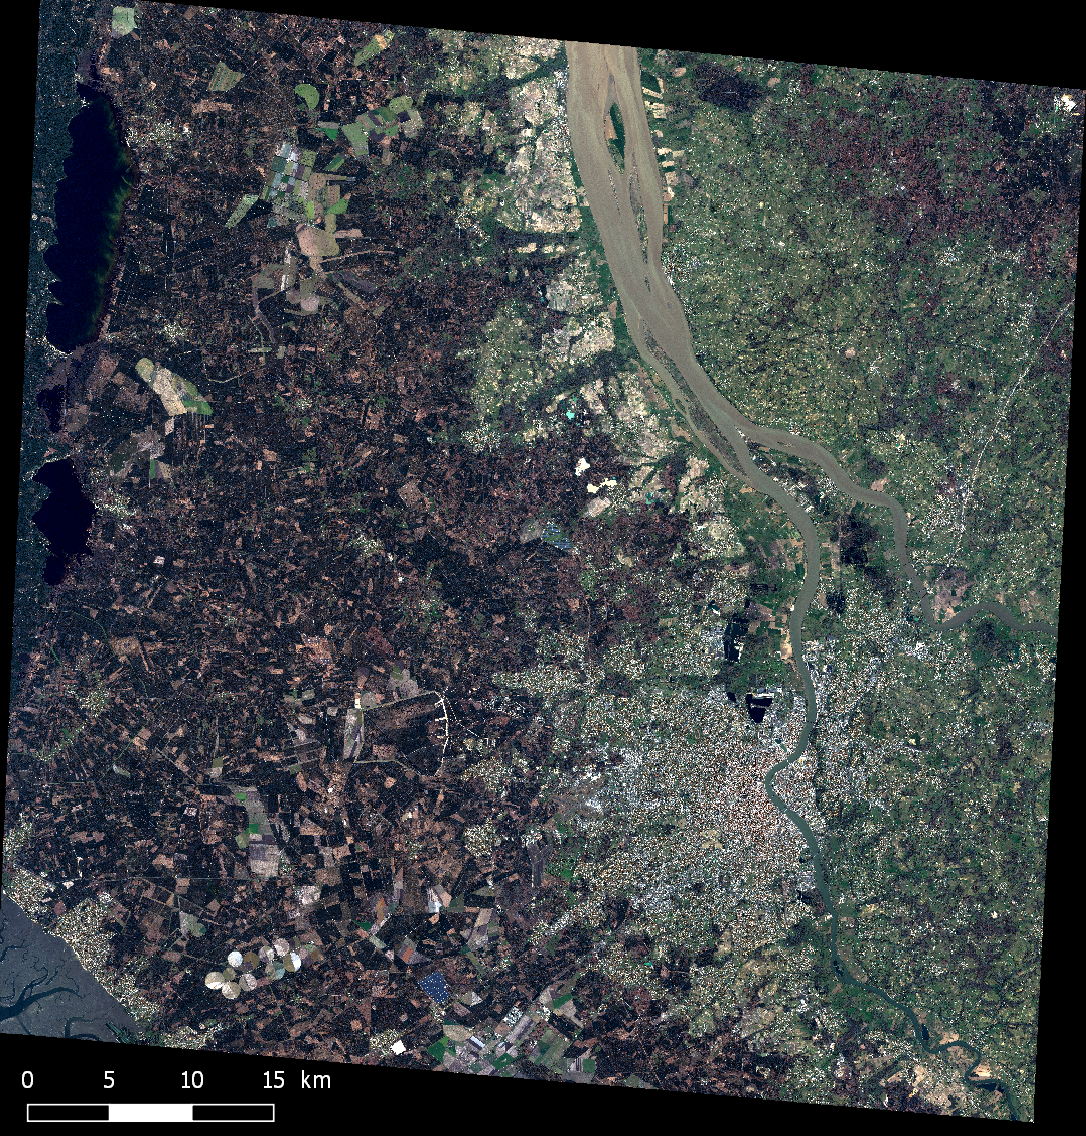
\includegraphics[width=.31\textwidth]{images/samples/gironde}
							}
							{
								\caption*{\tiny Image de la Gironde prise par SPOT en 2016: Résolution 1.5m, 4 canaux: \{{\color{purple!20}Infrarouge}, {\color{red}Rouge}, {\color{green}Vert}, {\color{blue}Bleu}\}.}
							}
							\ffigbox[\FBwidth]
							{
								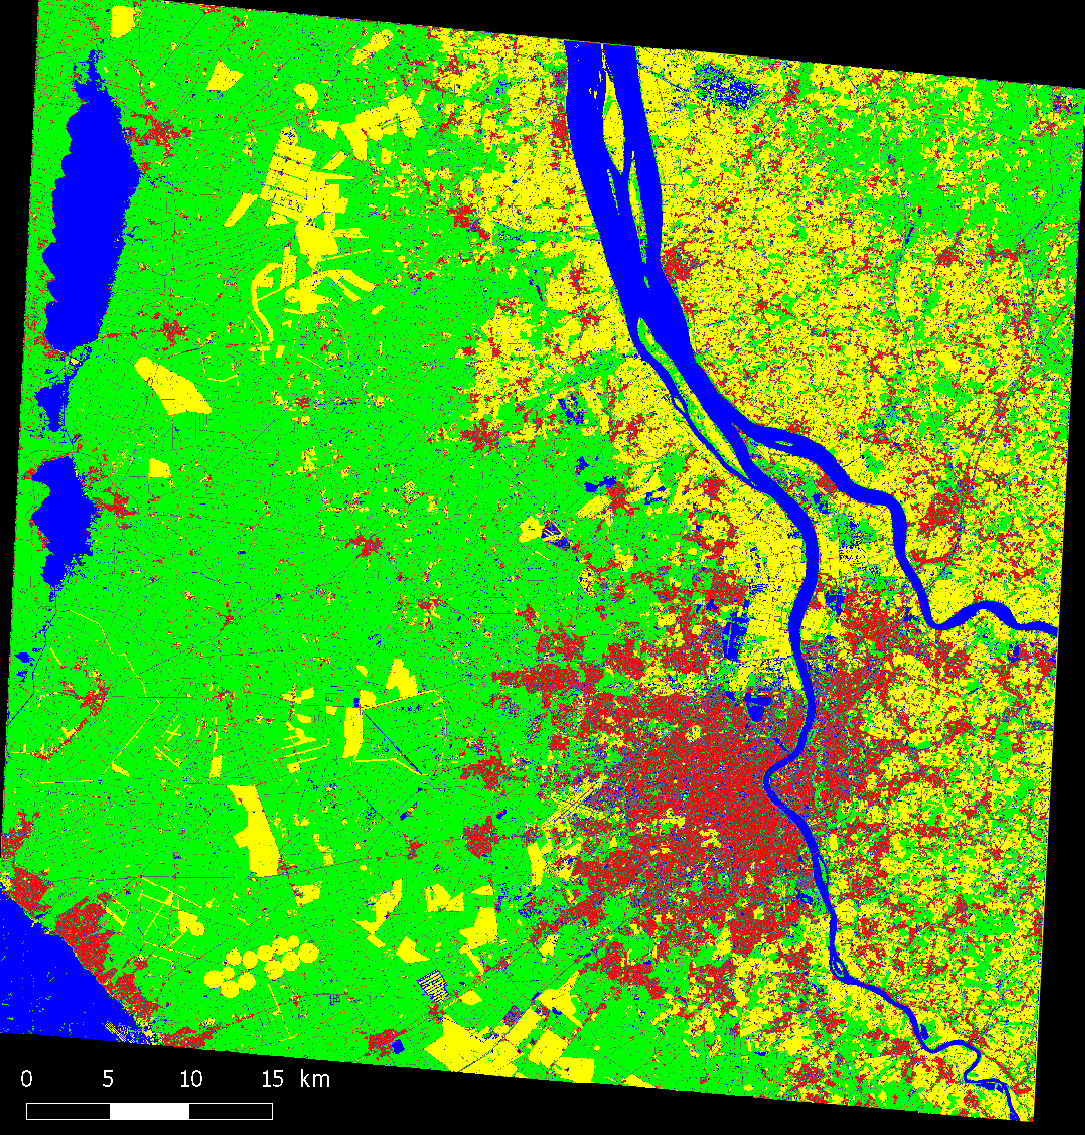
\includegraphics[width=.31\textwidth]{images/samples/gironde_classif}
							}
							{
								\caption*{\tiny Occupation des sols extraite de l'image: {\color{red}\(\blacksquare\)} Bâti, {\color{green}\(\blacksquare\)} Forêt, {\color{yellow}\(\blacksquare\)} Culture, {\color{gray}\(\blacksquare\)} Routes, {\color{blue}\(\blacksquare\)} Eau.}
							}
						\end{subfloatrow}
					}
					{
						\caption*{\tiny Classification appliquée pour l'Occupation des sols~\cite{postadjian2017investigating}.}
					}
				\end{figure}
			\end{frame}

			\begin{frame}{Segmentation de nuage de points}
				\begin{figure}[H]
					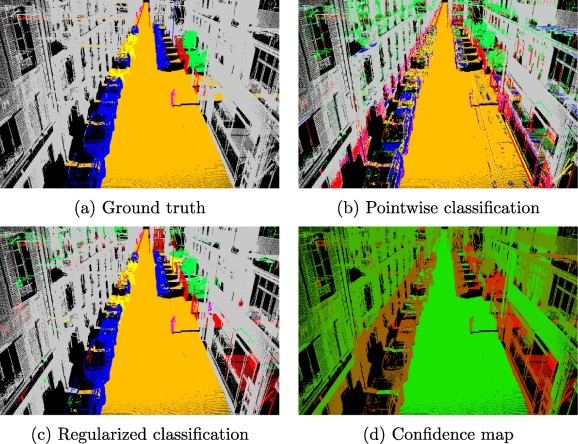
\includegraphics[width=.6\textwidth]{images/samples/pc_classification}
					\caption*{\tiny Exemple de classification de nuage de point\cite{landrieu2017structured}.}
				\end{figure}
			\end{frame}

			\begin{frame}{Détection de phénomènes}
				\begin{figure}[H]
					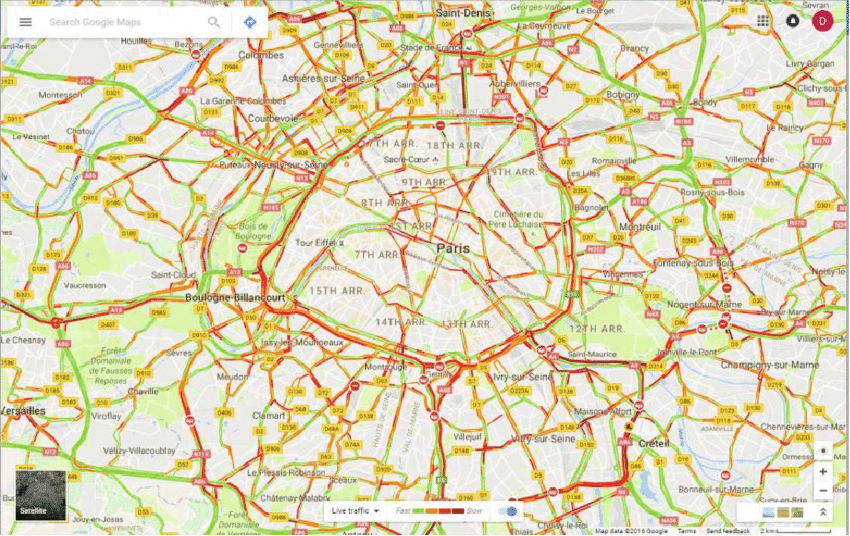
\includegraphics[width=.65\textwidth]{images/samples/traffic_paris}
					\caption*{\tiny Exemple de classification utilisé pour déterminer les conditions de circulation à Paris le 06/09/2016 à 9:30~\cite{tutic2016google}.}
				\end{figure}
			\end{frame}

			\begin{frame}{Classification avec RADAR}
				\begin{figure}[H]
					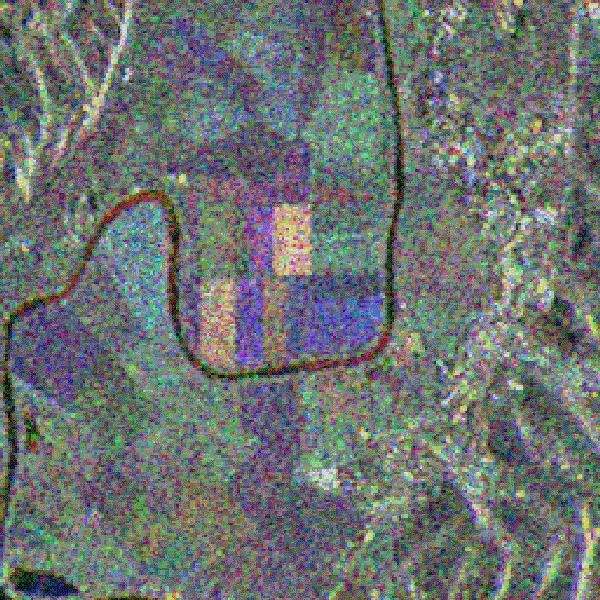
\includegraphics[width=.45\textwidth]{images/samples/radar}
					\caption*{\tiny Exemple d'occupation de sol utilisant basée RADAR~\cite{EsaRadar}.}
				\end{figure}
			\end{frame}

		\subsection{Observations}
			\begin{frame}{Comment caractériser les observations?}
				\begin{itemize}
					\item<1-> Comment sont représentés les données à classer?
					\item<2-> Quel est le point commun entre ces observations?
				\end{itemize}
			\end{frame}
		
			\begin{frame}{Observations}
				Les observations peuvent prendre beaucoup de formes:
				\begin{itemize}
					\item<2-> Image;
					\item<3-> Série temporelle (son, vidéo \dots);
					\item<4-> Graph de données;
					\item<5-> Nuage de points (LIDAR par exemple).
				\end{itemize}
			\end{frame}

			\begin{frame}{Attributs: représentation vectorielle}
				\begin{itemize}
					\item<1-> On représente généralement les observables par un vecteur dans \(\mathbb{R}^d\) qu'on nome attributs.
					\item<2-> On notera la \(i\)-ème observation par \(X^i = \begin{pmatrix}
						X^i_1\\
						X^i_2\\
						\vdots\\
						X^i_d
					\end{pmatrix}\).
					\item<3-> On notera donc l'ensemble des observations par \(\big( X^i \big)_{i=1,\dots, n}\).
				\end{itemize}
			\end{frame}

		\subsection{Types d'apprentissage}
			\begin{frame}{Apprentissage: supervisé et non-supervisé}
				Les classes peuvent être:
				\begin{itemize}
					\item<2-> non définies \(\longrightarrow\) apprentissage non-supervisé;
					\item<3-> définies \(\longrightarrow\) apprentissage (ou classification) supervisé.
				\end{itemize}
			\end{frame}

			\begin{frame}{Apprentissage supervisé}
				Dans le cas supervisé:
				\begin{itemize}
					\item<1-> Des classes sont définis \textit{a priori}: \(\{1,\dots, C\}\);
					\item<2-> Les observations sont divisée en deux ensembles:
						\begin{itemize}
							\item<3-> L'ensemble d'entraînement: chaque observation \(X^i, i=1,\dots,n_{train}\) a une classe \(Y^i \in \{1,\dots, C\}\);
							\item<4-> L'ensemble de test: des observations \(X^i, i=n_{train},\dots,n\) pour lesquels les classes \(Y^i, i=n_{train},\dots,n\) sont inconnues.
						\end{itemize}
					\item<5-> On ``apprend'' un modèle sur l'ensemble d'entraînement afin de prédire les classes \(Y^i, i=n_{train},\dots,n\) à partir des attributs \(X^i, i=n_{train},\dots,n\) seulement.
				\end{itemize}
			\end{frame}

			\begin{frame}{Apprentissage supervisé}
				\begin{figure}[H]
					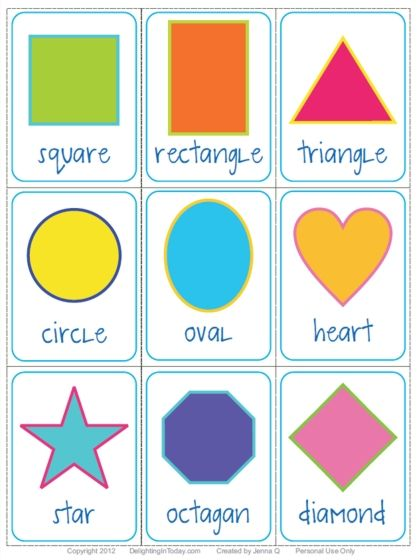
\includegraphics[height=.55\textheight]{images/samples/shapes_supervised}
					\caption*{Exemple de problème d'apprentissage supervisé: les classes (formes géométriques) sont données.}
				\end{figure}
			\end{frame}

			\begin{frame}{Apprentissage supervisé}
				Comment décrire les observations en forme de vecteur?
				\begin{itemize}
					\item<2-> nombre de côtés;
					\item<3-> nombre de sommets;
					\item<4-> convexité;
					\item<5-> symmetrie par rotation;
					\item<6-> \dots;
				\end{itemize}
				\uncover<7->{
					Pour une observation, dont la forme (classe) est un carré, le vecteur d'attributs s'écrit:
					\[\begin{pmatrix}
						4\\
						4\\
						True\\
						False\\
						\vdots
					\end{pmatrix}\]
				}
			\end{frame}

			\begin{frame}{Apprentissage supervisé}
				\begin{figure}[H]
					\begin{center}
						\includestandalone[mode=buildnew, height=.5\textheight]{scatter_gender_dataset}
						\caption*{\tiny Exemple de problème de classification supervisé: 2 attributs et 2 classes.}
					\end{center}
				\end{figure}
			\end{frame}

			\begin{frame}{Apprentissage non-supervisé}
				\begin{itemize}
					\item<1-> Dans le cas de l'apprentissage non-supervisé, on n'observe que les objets à classer, représentés par leurs attributs \(\big(X^i\big)_{i=1,\dots, n}\);
					\item<2-> Le but est de partitionner les instances en groupes (ou clusters) homgènes se ``ressemblent'' en un seul cluster;
					\item<3-> La ressemblance est basée sur les distances dans l'espace des attributs;
					\item<4-> La partition guarantie:
						\begin{itemize}
							\item<5-> des distances faibles intra-cluster;
							\item<6-> des distances grandes intra-cluster.
						\end{itemize}
				\end{itemize}
			\end{frame}

			\begin{frame}{Apprentissage non-supervisé}
				\begin{figure}[H]
					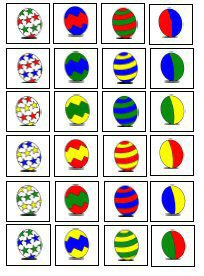
\includegraphics[height=.6\textheight]{images/samples/easter_non_supervised}
					\caption*{Exemple de problématique d'apprentissage non-supervisé.}
				\end{figure}
			\end{frame}

			\begin{frame}{Apprentissage supervisé}
				Comment décrire les observations en forme de vecteur?
				\begin{itemize}
					\item<2-> nombre de côté du motif régulier;
					\item<3-> couleur rouge;
					\item<4-> couleur verte;
					\item<5-> couleur blanche;
					\item<6-> couleur bleue;
					\item<7-> couleur jaune;
					\item<8-> couleur orange;
					\item<9-> convexité du motif;
					\item<10-> symmetrie par rotation du motif;
					\item<11-> symmetrie par translation du motif;
					\item<12-> \dots;
				\end{itemize}
				\uncover<13->{
					Pour l'instance en haut à droite, le vecteur d'attributs s'écrit:
					\[\begin{pmatrix}
						5 & 1 & 1 & 1 & 0 & 0 & 0 & False & False & False \dots
					\end{pmatrix}^T\]
				}
			\end{frame}

			\begin{frame}{Apprentissage non-supervisé}
				\begin{figure}[H]
					\begin{center}
						\includestandalone[mode=buildnew, height=.5\textheight]{scatter_circles}
						\caption*{\tiny Exemple de problème non-supervisé: 2 attributs. Les classes ne sont pas données mais une structure se dégage.}
					\end{center}
				\end{figure}
			\end{frame}

			\begin{frame}{Apprentissage non-supervisé}
				\begin{figure}[H]
					\begin{center}
						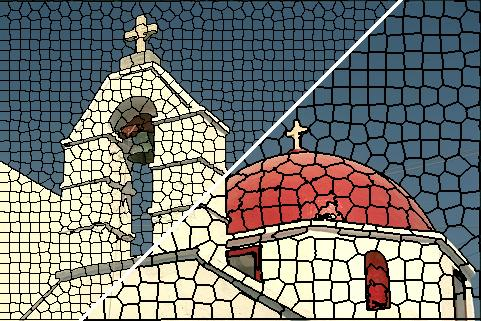
\includegraphics[height=.5\textheight]{images/samples/superpixels}
						\caption*{\tiny Exemple de problème non-supervisé: super-pixelisation d'une image~\cite{achanta2012slic}.}
					\end{center}
				\end{figure}
			\end{frame}
	\section{Algorithmes non-supervisé}
		\subsection{L'inertie}
			\begin{frame}{Variance intraclasse}
				\begin{itemize}
					\item<1-> Soit \(\big(S_k\big)_{k = 1, \dots, K}\) une \(K\)-partition de \(\{1, 2, \dots, n\}\).
					\item<2-> Pour chaque sous-ensemble \(S_k\), on définit la quantité \(\sum_{i\in S_k} d(X^i, \mu_k)^2\) où:
						\begin{itemize}
							\item<3-> \(d: \mathbb{R}^d \times \mathbb{R}^d \rightarrow \mathbb{R}_+\) représente une distance: dans tout ce qui suit \(d(x, y) = \lVert x - y \rVert\);
							\item<3-> \(\mu_k\) est le barycentre de \(S_k\): \( \mu_k \triangleq \frac{1}{\vert S_k \vert}.\sum_{i\in S_k} X^i\).
						\end{itemize}
					\item<4-> Cette quantité exprime la variance intraclasse.
				\end{itemize}
			\end{frame}
			\begin{frame}{Variance intraclasse}
				\begin{itemize}
					\item<1-> On suppose que la variable aléatoire \(Z: \Omega \rightarrow \mathbb{R}^d\) est telle que \(\mathbb{E}(Z) < \infty\) et \(\mathbb{E}(\lVert Z \rVert^2) < \infty\).
					\item<2-> \(\big(Z^i\big)_{i=1,\dots,p}\) sont \(p\) réaisations indépendentes et identiquement distribuées de même loi que \(Z\).
					\item<3-> Par définition, la variance empirique de \(\big(Z^i\big)_{i=1,\dots,p}\) est:
						\begin{equation}
							\text{Var}_{emp}(\big(Z^i\big)_{i=1,\dots,p}) \triangleq \frac{1}{p} . \sum_{i=1}^{p} \lVert Z^i - \bar Z \rVert^2 \underset{p\infty}{\longrightarrow} \text{Var}(Z) = \mathbb{E}(\lVert Z - \mathbb{E}(Z) \rVert^2)
						\end{equation}
						où \(\bar Z := \frac{1}{p}.\sum_{i=1}^{p} Z^i \underset{p\infty}{\longrightarrow} \mathbb{E}(Z)\).
					\item<4-> La disparité intraclasse vérifie donc bien évidemment:
						\begin{equation}
							\sum_{i\in S_k} \lVert X^i - \mu_k \rVert^2 = \vert S_k \vert . \text{Var}_{emp}(S_k)
						\end{equation}
						On voit bien que cette quantité exprime la variance des instances qui appartient au cluster \(S_k\).
				\end{itemize}
			\end{frame}
			\begin{frame}{Variance intraclasse}
				\begin{itemize}
					\item<1-> On remarque aussi que:
						\only<1>{
							\scriptsize
							\begin{align*}
								\sum_{i,j\in S_k} \lVert X^i - X^j \rVert^2 &= \sum_{i,j\in S_k} \lVert (X^i -\mu_k) + (\mu_k - X^j) \rVert^2\\
																			&= \sum_{i,j\in S_k} \lVert X^i -\mu_k \rVert^2 + \lVert \mu_k - X^j \rVert^2 + 2 . \langle X^i -\mu_k , \mu_k - X^j \rangle\\
																			&= \sum_{i,j\in S_k} \lVert X^i -\mu_k \rVert^2 + \sum_{i,j\in S_k} \lVert \mu_k - X^j \rVert^2 + 2. \sum_{i,j\in S_k} \langle X^i -\mu_k , \mu_k - X^j \rangle\\
																			&= \vert S_k \vert . \sum_{i\in S_k} \lVert X^i -\mu_k \rVert^2 + \vert S_k \vert . \sum_{j\in S_k} \lVert X^j -\mu_k \rVert^2 + 2 . \langle \sum_{i\in S_k}(X^i -\mu_k) , \sum_{j\in S_k} (\mu_k - X^j) \rangle\\
																			&= 2. \vert S_k \vert . \sum_{i\in S_k} \lVert X^i -\mu_k \rVert^2 + 2.\langle \cancelto{0}{\sum_{i\in S_k} X^i - \vert S_k \vert.\mu_k}, \cancelto{0}{\vert S_k \vert.\mu_k - \sum_{j\in S_k} X^j}\rangle\\
																			&= 2. \vert S_k \vert . \sum_{i\in S_k} \lVert X^i -\mu_k \rVert^2
							\end{align*}
						}
						\uncover<2->{
							\begin{equation}
								\sum_{i,j\in S_k} \lVert X^i - X^j \rVert^2 = 2. \vert S_k \vert . \sum_{i\in S_k} \lVert X^i -\mu_k \rVert^2
							\end{equation}
						}
					\item<3-> Cette équation lie, proportionellement, le premier terme décrivant l'hétérogénité de l'ensemble \(S_k\) avec le deuxième qui exprime la variance intraclasse.
				\end{itemize}
			\end{frame}

			\begin{frame}{Inertie intraclasse}
				\begin{itemize}
					\item<1-> On somme les différentes disparités intra-cluster sur tout les sous-ensembles \(S_k\). On définit l'inertie intraclasse de la partition:
						\begin{equation}
							I_W(\big(S_k\big)_{k = 1, \dots, K}) \triangleq \sum_{k= 1}^{K} \sum_{i\in S_k} d(X^i, \mu_k)^2
						\end{equation}
					\item<2-> Pour le cas particulier de \(K=1\), on vérifie \(\big(S_k\big)_{k = 1, \dots, K} = (\{1,\dots,n\})\). On définit donc l'inertie totale des instances:
						\begin{equation}
							I_T \triangleq \sum_{i=1}^{n} d(X^i, \mu)^2
						\end{equation}
						avec \(\mu = \frac{1}{n} . \sum_{i=1}^{n} X^i\).
				\end{itemize}
			\end{frame}

			\begin{frame}[allowframebreaks]{Inertie totale}
				\begin{align*}
					I_T &= \sum_{i=1}^{n} \lVert X^i - \mu \rVert^2\\
						&= \sum_{k= 1}^{K} \sum_{i\in S_k} \lVert X^i - \mu \rVert^2\\
						&= \sum_{k= 1}^{K} \sum_{i\in S_k} \lVert X^i - \mu_k \rVert^2 + \lVert \mu_k - \mu \rVert^2 + 2. \langle X^i-\mu_k, \mu_k-\mu \rangle\\
						&= I_W(\big(S_k\big)_{k = 1, \dots, K}) + \sum_{k= 1}^{K} \sum_{i\in S_k} \lVert \mu_k - \mu \rVert^2 + 2 . \sum_{k= 1}^{K} \sum_{i\in S_k} \langle X^i-\mu_k, \mu_k-\mu \rangle\\
						&= I_W(\big(S_k\big)_{k = 1, \dots, K}) + \sum_{k= 1}^{K} \vert S_k \vert \lVert \mu_k - \mu \rVert^2 + 2 . \sum_{k= 1}^{K} \langle \sum_{i\in S_k} (X^i-\mu_k), \mu_k-\mu \rangle
				\end{align*}
				\begin{align*}
					I_T &= I_W(\big(S_k\big)_{k = 1, \dots, K}) + \sum_{k= 1}^{K} \vert S_k \vert \lVert \mu_k - \mu \rVert^2 + 2 . \sum_{k= 1}^{K} \langle \sum_{i\in S_k} X^i - \vert S_k \vert . \mu_k, \mu_k-\mu \rangle\\
						&= I_W(\big(S_k\big)_{k = 1, \dots, K}) + \sum_{k= 1}^{K} \vert S_k \vert \lVert \mu_k - \mu \rVert^2 + 2 . \sum_{k= 1}^{K} \langle \sum_{i\in S_k} X^i - \vert S_k \vert . \frac{1}{\vert S_k \vert} . \sum_{i\in S_k} X^i, \mu_k-\mu \rangle\\
						&= I_W(\big(S_k\big)_{k = 1, \dots, K}) + \sum_{k= 1}^{K} \vert S_k \vert \lVert \mu_k - \mu \rVert^2
				\end{align*}
			\end{frame}

			\begin{frame}{Inertie interclasse}
				\begin{itemize}
					\item<1-> On définit ainsi l'inertie interclasse:
						\begin{equation}
							I_B(\big(S_k\big)_{k = 1, \dots, K}) = \sum_{k= 1}^{K} \vert S_k \vert \lVert \mu_k - \mu \rVert^2
						\end{equation}
						on a donc:
						\begin{equation}
							I_T = I_B(\big(S_k\big)_{k = 1, \dots, K}) + I_W(\big(S_k\big)_{k = 1, \dots, K})
						\end{equation}
					\item<2-> Cette quantité \(I_B\) exprime la disparité entre les barycentre de cluster et le barycentre de tous les échantillons. Plus elle est grande, plus l'hétérogénité de la partition est grande.
					\item<3-> Puisque \(I_T\) est constante, minimiser la disparité intra-cluster \(I_W\) revient à maximiser \(I_B\).
					\item<4-> Trouver la meilleure partition revient à résoudre le problème:
						\begin{equation}
							\arg \min_{\substack{K = 1,\dots,n \\ \big(S_k\big)_{k = 1, \dots, K}}} I_W(\big(S_k\big)_{k = 1, \dots, K})
						\end{equation}
				\end{itemize}
			\end{frame}

			\begin{frame}{Combinatoire}
				\begin{itemize}
					\item<1-> A premier abord, on peut essayer toutes les partitions possibles.
					\item<2-> Pour \(n\) instances et \(K\) classes, le nombre totale de partition~\cite{StirlingWiki}:
						\begin{equation}
							S_{n,K} \triangleq \left\{ {n \atop k}\right\} = \frac{1}{k!}\sum_{j=0}^{k} (-1)^{k-j} \binom{k}{j} j^n
						\end{equation}
					\item<3-> Pour \(k \neq 1, n\):
						\begin{equation}
							S_{n,K} \underset{n\infty}{\sim} \frac{K^n}{K!}
						\end{equation}
					\item<4-> Pour toute les partitions possibles, on dénombre:
						\begin{equation}
							B_n \triangleq \sum_{k=0}^n \left\{ {n \atop k}\right\} = \frac{1}{e}\sum_{k\in\mathbb{N}} \frac{k^n}{k!}
						\end{equation}
						avec: \(\frac{B_n}{n^n} \underset{n\infty}{\sim} 1\)~\cite{BellWiki}.
				\end{itemize}
			\end{frame}
		\subsection{Clustering hiérarchique}
			\begin{frame}{Clustering hiérarchique}
				\begin{itemize}
					\item<1-> On repose sur la métrique \(d\) qui repose sur la géométrie dans l'espace des attributs.
					\item<2-> On définit une distance entre clusters:
						\begin{itemize}
							\item<3-> \(D_m: (A, B) \mapsto \min_{a\in A, b\in B} d(a,b)\)
							\item<4-> \(D_M: (A, B) \mapsto \max_{a\in A, b\in B} d(a,b)\)
							\item<5-> \(D_b: (A, B) \mapsto \frac{1}{\vert A \vert.\vert B \vert}\sum_{a\in A, b\in B} d(a,b)\)
							\item<6-> \dots
						\end{itemize}
					\item<7-> On regroupe (\textit{resp.} divise) les clusters qui vérifient le minimum (\textit{resp.} maximum) de distance~\cite{hastie2009unsupervised,ward1963hierarchical}.
				\end{itemize}
			\end{frame}
			\begin{frame}{Exemple}
				\begin{figure}[H]
					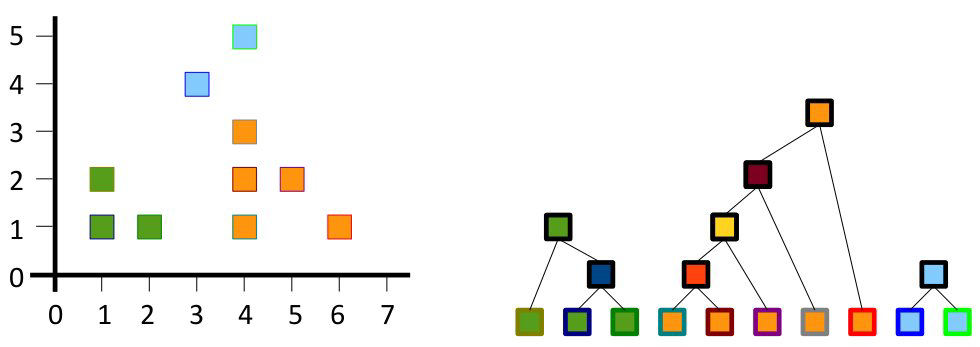
\includegraphics[width=.8\textwidth]{images/samples/hierchical_clustering.png}
					\caption*{Exemple de clustering hiérarchique}
				\end{figure}
			\end{frame}
			\begin{frame}{Algorithme}
				\begin{algorithm}[H]
					\KwData{Les observations: \(\big(X^i\big)_{i=1,\dots,n}\)}
					\KwData{La métrique de cluster: \(D: 2^{\{X^i: i=1,\dots,n\}} \times 2^{\{X^i: i=1,\dots,n\}} \rightarrow \mathbb{R}_+\)}
					\KwData{Le nombre d'itération maximale: \(I\)}
					\KwData{Le nombre de clusters: \(K\)}
					
					\KwResult{Le nombre de clusters: \(cl\) et la partition: \(\big(S_k\big)_{k=1,\dots,cl}\)}
					\(t := 0\), \(S^t_k:=\{X^k\}, \quad \forall k = 1,\dots,n\), \(cl=n\)\;
					\While{\(cl > K\) and \(t < I\)}{
						\(t := t + 1\)\;
						Couples à regrouper: \(\big\{c_1, \dots, c_{p_t}\big\} := \arg\min_{\substack{s=1,\dots,cl\\t=1,\dots,cl}} D(S^{t-1}_s, S^{t-1}_t)\)\;
						Ensembles à regrouper: \(\{e_1,\dots,e_{q_t}\} := \big\{\bigcup_{\substack{k=1,\dots,p_t\\c_j\cup c_k \neq \emptyset}} c_k: j=1,\dots,p_t\big\}\)\;
						Regroupement: \(\forall k=1,\dots,q_t \quad S^t_k := \bigcup_{j\in e_k} S^{t-1}_j\)\;
						Cluster inchangés: \(\big\{S^t_k: k=q_t+1,\dots,cl\} := \{S^{t-1}_h: h\in\{1,\dots,cl\} \setminus \bigcup_{j=1}^{q_t} e_j \big\}\)\;
						Nombre de clusters: \(cl:= cl + q_t - \sum_{j=1}^{q_t} \vert e_i\vert\)\;
					}
				\end{algorithm}
			\end{frame}

		\subsection{Clustering avec partitionnement}
			\begin{frame}{K-means}
				\begin{itemize}
					\item<1-> On suppose que \(K\) le nombre de classes possibles est fixe.
					\item<2-> On rappelle le problème d'optimisation à résoudre dans ce cas:
						\begin{equation}
							\arg \min_{\big(S_k\big)_{k = 1, \dots, K}} \sum_{k= 1}^{K} \sum_{i\in S_k} \lVert X^i - \mu_k\rVert^2
						\end{equation}
					\item<3-> La complexité en temps pour la résolution de ce problème est \(O(n^{d.K+1})\)~\cite{inaba1994applications}.
					\item<4-> Elle est exponentielle en dimension \(d\) (curse of dimensionality) et en \(K\).
					\item<5-> Il faut trouver une heuristique qui est linéaire dans la plupart des cas.
				\end{itemize}
			\end{frame}
			\begin{frame}{Algorithme de Loyd}
				\begin{algorithm}[H]
					\KwData{Les observations: \(\big(X^i\big)_{i=1,\dots,n}\)}
					\KwData{Le nombre d'itération maximale: \(I\)}
					\KwData{Le nombre de clusters: \(K\)}

					\KwResult{La partition: \(\big(S_k\big)_{k=1,\dots,K}\)}
					\(t := 0\), \(\forall k = 1,\dots,K \quad \mu^t_k := X^{random(\{1,\dots,n\})}\)\;
					\Do{\(t < I\) and \(\forall k=1,\dots,K \quad \Delta_t\mu_k \neq 0\)}{
						\(t := t + 1\)\;
						Assignement: \(\forall k = 1,\dots,K \quad S_k := \arg \min_{i=1,\dots,n} \lVert X^i - \mu^{t - 1}_k \rVert\)\;
						Mise à jour: \(\forall k = 1,\dots,K \quad \mu^t_k := \frac{1}{\vert S_k \vert}.\sum_{j \in S_k} X^j\)\;
					}
				\end{algorithm}
			\end{frame}
			\begin{frame}{K-means}
				\begin{itemize}
					\item[\color{green}+]<1-> Algorithme simple à implémenter;
					\item[\color{green}+]<1-> En général, faible complexité en temps: \(O(n.d.K.I)\);
					\item[\color{red}-]<2-> Convergence vers un minimum local;
					\item[\color{red}-]<2-> Nécessité de la connaissance \textit{a priori} de \(K\);
					\item[\color{red}-]<2-> Inadéquation de la métrique Euclidienne.
				\end{itemize}
			\end{frame}
			\begin{frame}{ISODATA}
				\begin{itemize}
					\item<1-> \(K\) n'est pas fixé.
					\item<2-> Comme le K-moyennes, sauf qu'on peut regrouper les clusters qui se ressemblent ou diviser ceux qui sont trop hétérogène.
					\item<3-> Le critère d'arrêt repose sur:
						\begin{itemize}
							\item<3-> La moyenne de la distance entre centroïdes passe en dessous d'un seuil;
							\item<4-> La moyenne du changement de l'inertie intraclasse est en dessous d'un seuil;
							\item<5-> Le nombre maximale des itérations est atteint.
						\end{itemize}
				\end{itemize}
			\end{frame}
			\begin{frame}{ISODATA}
				\begin{algorithm}[H]
					\KwData{Les observations: \(\big(X^i\big)_{i=1,\dots,n}\)}
					\KwData{Le nombre d'itération maximale: \(I\)}
					\KwData{Le nombre de clusters: \(K\)}
					\KwData{Le seuil de regroupement: \(s_g\)}
					\KwData{Le seuil d'éclatement: \(s_e\)}
					\KwData{La tolérance de la disparité des centres: \(T_c\)}
					\KwData{La tolérance de changement d'inertie: \(T_i\)}					

					\KwResult{Le nombre de clusters: \(K\) et la partition: \(\big(S_k\big)_{k=1,\dots,K}\)}
					\(t := 0\), \(K^t := random(\{1,\dots,n\})\), \(\forall k = 1,\dots,K^t \quad \mu^t_k := X^{random(\{1,\dots,n\})}\)\;
					\Do{\(t < I\) and \(\max_{\substack{k=1,\dots,K\\l=1,\dots,K}} d(\mu^t_l, \mu^t_k) > T_c \) and \(\Delta_t I_W(\big(S^t_k\big)_{k = 1, \dots, K}) > T_i\)}{
						\(t := t + 1\)\;
						Assignement: \(\forall k = 1,\dots,K^{t-1} \quad S^t_k := \arg \min_{i=1,\dots,n} \lVert X^i - \mu^{i - 1}_k \rVert\)\;
						Regroupement: \(R := \{\bigcup_{\substack{l = 1,\dots,K^{t-1}\\ \lVert\mu_l - \mu_k\rVert \leq s_g}} S^{t-1}_l: k=1,\dots,K^{t-1}\}\)\;
						Eclatement: \(\{S_1, \dots, S_{K^t}\} := \bigcup\{eclate(r): r \in R\}\)\;
						Mise à jour: \(\forall k = 1,\dots,K^t \quad \mu^t_k := \frac{1}{\vert S^t_k \vert}.\sum_{j \in S^t_k} X^j\)\;
					}
				\end{algorithm}
			\end{frame}
			\begin{frame}{ISODATA}
				\begin{itemize}
					\item[\color{green}+]<1-> Algorithme simple à implémenter;
					\item[\color{green}+]<1-> Moins d'\textit{a priori};
					\item[\color{red}-]<2-> Convergence vers un minimum local: généralement \(K = 1\);
					\item[\color{red}-]<2-> Nécessité de la connaissance de plusieur seuils;
					\item[\color{red}-]<2-> Inadéquation de la métrique Euclidienne.
				\end{itemize}
			\end{frame}

	\section{Algorithmes supervisés}
		\subsection{Formalisation}
			\begin{frame}{Fonction de décision}
				\begin{itemize}
					\item<1-> On suppose que ${\big((X^i, Y^i)\big)}_{i=1,\dots,n}$ sont des réalisations indépendantes et identiquement distribuées (i.i.d) de la loi $\mathbb{P}(X=x, Y=y) = p(x,y)$.
					\item<2-> On cherche une fonction de décision $D$ comme suit:
					\begin{align*}
						D: \mathbb{R}^d &\rightarrow \{1, \dots, C\} \\
						x &\mapsto D(x)
					\end{align*}
					\item<3-> On définit le regret, ou risque, d'une fonction de décision $D$ par:
					\begin{equation}
						R(D) \triangleq \mathbb{E}_{X,Y}(\mathbb{1}(D(X)\neq Y))
					\end{equation}
					\item<4-> Cette fonction calcule la mesure de l'espace d'attributs où $D(x) \neq y$:
					\begin{align*}
						R(D) &= \mathbb{P}(\{D(X)\neq Y\})\\
							&= \sum_{y\in \{-1, 1\}} \int_{x \in \mathbb{R}^d} \mathbb{1}(D(x)\neq y) p(dx, y)
					\end{align*}
				\end{itemize}
			\end{frame}
			\begin{frame}{Risque empirique}
				\begin{itemize}
					\item<1-> Le risque empirique est défini par:
						\begin{equation}
							R_n(D) \triangleq \sum_{i=1}^n \mathbb{1}_{D(X^i) \neq Y^i} \underset{n\infty}{\longrightarrow} R(D)
						\end{equation}
					\item<2-> Soit \(D^*\) la fonction de décision optimale. Elle vérifie:
						\begin{equation}
							D^* \triangleq \arg\min_{D \in \mathscr{F}} R(D)
						\end{equation}
					\item<3-> Soit \(\widehat D \) la fonction de décision empirique optimale:
						\begin{equation}
							\widehat D \triangleq \arg\min_{D \in \mathscr{F}} R_n(D)
						\end{equation}
					\item<3-> Exemple d'ensemble de recherche: \(\mathscr{F} = \{1, \dots, C\}^{\mathbb{R}^d}\) l'ensemble de toute les fonctions possibles.
					\item<4-> Ce dernier choix est trop naif. En effet, on défini la fonction de décision \(D_{naïve}: x \mapsto \sum_{i=1,\dots,n} Y^i . \delta_{X^i}(x) + \mathbb{1}_{x \notin \{X^i, \forall i=1,\dots,n\}}\). On observe que \(R_n(D_{naïve}) = 0\).
				\end{itemize}
			\end{frame}
			\begin{frame}{Sur/Sous apprentissage}
				\begin{itemize}
					\item<1-> On quantifie la différence de \(\widehat D \) par rapport à \(D^*\) par:
						\begin{equation}
							R(D^*) - 
						\end{equation}
					\item<2-> Bias Variance decomp
				\end{itemize}
			\end{frame}
			\begin{frame}{Sur/Sous apprentissage}
				\begin{itemize}
					\item<1-> On quantifie la différence de \(\widehat D \) par rapport à \(D^*\) par:
						\begin{equation}
							R(D^*) - 
						\end{equation}
					\item<2-> Bias Variance decomp
				\end{itemize}
			\end{frame}
			\begin{frame}{Sur/Sous apprentissage}
				\begin{figure}[H]
					\includestandalone[mode=buildnew, width=.5\textwidth]{scatter_separators}
					\caption*{Illustration des cas de sur/sous apprentissage.}
				\end{figure}
			\end{frame}
			\begin{frame}{Discriminatif vs Génératif}
				\begin{itemize}
					\item<1-> On sait modéliser la distribution des classes $p(y)$ et celle des instances selon la classe $p(x\vert y)$ $\longrightarrow$ méthode générative,
						\begin{itemize}
							\item<2-> Exemple: On s'interresse à la détection de sexe selon deux mesures: taille et poids.
							\item<3-> On suppose que la répartition des sexes est équilibrée dans le monde $p(y=1) = p(y=0) = \frac{1}{2}$;
							\item<4-> la répartition des mesures suivent des lois gaussiennes $X\vert Y=y \sim \mathscr{N}(m_y, \sigma_y)$.
						\end{itemize}
					\item<5-> On n'a aucune connaissance \textit{a priori}. On cherche à apprendre un modèle de $p(y \vert x)$ $\longrightarrow$ méthode discriminative.
				\end{itemize}
			\end{frame}	
		\subsection{Méthodes génératives}
			\begin{frame}{Règle de Bayes}
				\begin{equation}
					p(y \vert x) = \frac{p(x \vert y).p(y)}{p(x)}
				\end{equation}
				\begin{itemize}
					\item $p(y)$ : probabilité d'appartenir à la classe $y$.
					\item $p(x)$ : probabilité que l'attribut $X=x$.
					\item $p(x \vert y)$  : probabilité que $X=x$ pour la classe $y$.
					\item $p(y \vert x)$  : probabilité d'appartenir à la classe $y$ sachant que $X=x$.
				\end{itemize}
			\end{frame}
			\begin{frame}{La classe estimée}
				\begin{itemize}
					\item<1-> La classe estimée \(D(x)\) est la classe la plus probable sachant $X=x$: 
						\begin{equation}
							D(x) = \arg \max_{y=1,\dots,C} p(y \vert x)
						\end{equation}
					\item<2-> Dans le cas génératif, on a donc:
						\begin{align}
							D(x) &= \arg \max_{y=1,\dots,C} \frac{p(x \vert y).p(y)}{p(x)}\\
							D(x) &= \arg \max_{y=1,\dots,C} p(x \vert y).p(y)
						\end{align}
				\end{itemize}
			\end{frame}
			\begin{frame}{Exemple: Tennis or no Tennis}
				\begin{table}[H]
					\begin{center}
						\begin{tabular}{c c c c c}
							\toprule
							Temps (C) & Température (T) & Humidité (H) & Vent (V) & Tennis\\
							\midrule
							soleil & chaud & élevée & non & non\\
							soleil & chaud & élevée & oui & non\\
							couvert & chaud & élevée & non & oui\\
							pluie & tiède & élevée & non & oui\\
							pluie & froid & normale & non & oui\\
							pluie & froid & normale & oui & non\\
							couvert & froid & normale & oui & oui\\
							soleil & tiède & élevée & non & non\\
							soleil & froid & normale & non & oui\\
							pluie & tiède & normale & non & oui\\
							soleil & tiède & normale & oui & oui\\
							couvert & tiède & élevée & oui & oui\\
							couvert & chaud & normale & non & oui\\
							\bottomrule
						\end{tabular}
					\end{center}
				\end{table}
			\end{frame}
			\begin{frame}{Exemple: Tennis or no Tennis}
				\begin{itemize}
					\item \(p(Tennis = oui) = \frac{9}{14}\) et \(p(Tennis = non) = \frac{5}{14}\);
					\item On suppose que les différentes mesures de climats sont indépendantes \(P((C, T, H, V) \vert Tennis) = P(C\vert Tennis).P(T\vert Tennis).P(H\vert Tennis).P(V\vert Tennis)\);
					\item Application numérique pour \(X=(pluie, chaud,\)\textit{élevée}\(, non)\): 
						\[p(Tennis = oui \vert X) = p(X\vert Tennis = oui) . p(Tennis = oui) \approx 0.010582\]
						\[p(Tennis = non \vert X) = p(X\vert Tennis = non) . p(Tennis = non) \approx \boldmath 0.018286\]
						Donc quand il pleut, il fait chaud, la température est élevée et il n'y a pas de vent, on ne joue pas.
				\end{itemize}
			\end{frame}
		\subsection{Méthodes discriminative}
			\begin{frame}{Méthodes de centroïdes}
				\begin{itemize}
					\item<1-> On s'inspire du clustering: On assigne la classe dont le centroïde est le plus proche.
					\item<2-> On pose \(\mu_k = \frac{1}{\vert \{i\in\{1,\dots,n\}: Y^i = k\} \vert}.\sum_{\substack{i=1,\dots,n\\Y^i = k}} X^i\). On peut écrire:
						\begin{equation}
							D_{centroid}(x) \triangleq \arg \min_{k=1,\dots,C} \lVert x - \mu_k \rVert
						\end{equation}
				\end{itemize}
			\end{frame}
			\begin{frame}{Méthodes de centroïdes}
				\begin{figure}[H]
					\includestandalone[mode=buildnew, height=.5\textheight]{scatter_circles_class}
					\caption*{Problème de la méthode de centroïde. Les deux classes sont cocentriques.}
				\end{figure}
			\end{frame}
			\begin{frame}{k-NN}
				\begin{itemize}
					\item<1-> On choisit les \(k\) instances les plus proches de l'observation \(x\). On assigne à cette observation la classe majoritaire parmi les \(k\) classes de ces voisins.
					\item<2-> Soit \(o_1,\dots,o_n\) les indices qui guarantissent: \(\lVert x - X^{o_1} \rVert \leq \lVert x - X^{o_2} \rVert \dots \leq \lVert x - X^{o_n} \rVert\). Les \(k\) plus proches voisins sont donc \(\{X^{o_1}, X^{o_2},\dots,X^{o_k}\}\).
					\item<3-> On définit donc la fonction de décision du k-NN par:
						\begin{equation}
							D_{knn}(x) \triangleq \arg \max_{c=1,\dots,C} \sum_{i=1,\dots,k} \mathbb{1}_{Y^{o_i} = c}
						\end{equation}
					\item<4-> Plus k augmente, plus les frontières seront lisses.
				\end{itemize}
			\end{frame}
			\begin{frame}{Arbres de décision}
				\begin{figure}[H]
					\includestandalone[mode=buildnew, width=.7\textwidth]{decision_tree}
					\caption*{Exemple d'arbre de décision.}
				\end{figure}
			\end{frame}
			\begin{frame}{Forêts aléatoire}
				
			\end{frame}
	
	\section{Qualification des résultats}
		\subsection{}

	\section{Références}
	\begin{frame}[allowframebreaks]{Références}
		\bibliographystyle{apalike}
		\bibliography{references.bib}
	\end{frame}

\end{document}
